\documentclass[11pt]{article}
\usepackage{amsmath, amssymb, mathtools, bm}
\usepackage{physics}
\usepackage{tikz, pgfplots}
\pgfplotsset{compat=1.18}
\usepackage[margin=2.3cm]{geometry}
\usepackage{siunitx, booktabs, hyperref}

\newcommand{\D}{\mathrm{D}}
\newcommand{\de}{\mathrm{d}}
\newcommand{\pd}[2]{\frac{\partial #1}{\partial #2}}
\newcommand{\pdd}[2]{\frac{\partial^{2} #1}{\partial #2^{2}}}
\newcommand{\Lap}{\nabla^{2}}

\title{B1 Fluids --- Model Solutions, Trinity Term 2022}
\author{}
\date{}

\begin{document}
\maketitle

%==================================================================
\section*{Question 1 --- Darcy flow}

\textbf{Problem.} Stack of $n$ rigid sheets, gap $b\ll w,L$, fluid $(\rho,\eta)$, pressure drop $\Delta p$ across length $L$. Derive velocity field and Darcy permeability $\Pi_0$; comment on inertia. Then generalise, prove $\nabla\!\cdot\!(\rho\vb q)=0$, solve a spherical injection, compare two aquifers, and discuss gravity.

\subsection*{(a)}

Take $\hat{\vb x}$ along the plates, $z\in[0,b]$ across the gap. Symmetry and no-penetration:
\[ \vb u = u_x(z)\hat{\vb x}, \qquad u_y=u_z=0. \]
Steady, unidirectional, $z$-independent pressure: Navier--Stokes reduces to:
\[ 0 = -\pd{p}{x} + \eta\,\pdd{u_x}{z}, \qquad \pd{p}{z}=0. \]
Constant pressure gradient:
\[ \pd{p}{x} = -\frac{\Delta p}{L}. \]
Integrate twice in $z$:
\[ u_x(z) = -\frac{1}{2\eta}\frac{\Delta p}{L}\,z(b-z)\cdot(-1) + C_1 z + C_2. \]
Apply no-slip $u_x(0)=u_x(b)=0$:
\[ u_x(z) = \frac{\Delta p}{2\eta L}\,z(b-z). \]
Volume flux per unit cross-sectional area:
\[ q = \frac{1}{b}\int_0^b u_x\,\de z. \]
Evaluate the integral:
\[ q = \frac{\Delta p}{2\eta L b}\cdot\frac{b^3}{6} = \frac{b^2}{12\eta}\frac{\Delta p}{L}. \]
Compare with $q=(\Pi_0/\eta)(\Delta p/L)$:
\[ \boxed{\;\Pi_0 = \frac{b^2}{12}.\;} \]

\paragraph{Inertia.} For unidirectional $u_x(z)$: $(\vb u\cdot\nabla)\vb u = u_x\partial_x u_x\hat{\vb x}=0$ identically. Force balance is pressure $\leftrightarrow$ viscous stress only; inertia plays no role. Equivalently $\mathrm{Re}=Ub/\nu\ll 1$ in the Darcy regime.

\subsection*{(b)}

Mass conservation in fixed volume $V$:
\[ \dv{t}\!\int_V \rho\,\de V = -\oint_{\partial V}\rho\vb q\cdot\de\vb S. \]
Steady, rigid matrix: LHS$=0$. Apply divergence theorem:
\[ \int_V \nabla\!\cdot\!(\rho\vb q)\,\de V = 0. \]
Volume arbitrary, integrand continuous:
\[ \boxed{\;\nabla\!\cdot\!(\rho\vb q) = 0.\;} \]

\subsection*{(c)}

Spherically symmetric, $\rho$ constant, $\nabla\!\cdot\!\vb q=0$ with $\vb q=q_r(r)\hat{\vb r}$:
\[ \frac{1}{r^2}\dv{r}\!\left(r^2 q_r\right) = 0. \]
Integrate:
\[ q_r = \frac{C}{r^2}. \]
Darcy without gravity: $\vb q=-(\Pi_1/\eta)\nabla p$, so $q_r=-(\Pi_1/\eta)\,\de p/\de r$:
\[ \dv{p}{r} = -\frac{\eta C}{\Pi_1 r^2}. \]
Integrate from $r$ to $\infty$ with $p(\infty)=p_0$:
\[ p(r) - p_0 = \frac{\eta C}{\Pi_1 r}. \]
Apply $p(a)=p_0+\Delta p$:
\[ C = \frac{\Pi_1\,\Delta p\,a}{\eta}. \]
Hence:
\[ \boxed{\;q_r(r) = \frac{\Pi_1\,\Delta p\,a}{\eta\,r^2}.\;} \]

\paragraph{Aquifer choice.} Pump power at fixed flow rate $Q=4\pi a^2 q_r(a)$:
\[ Q = \frac{4\pi a\,\Pi_1\,\Delta p}{\eta}. \]
Invert for $\Delta p$:
\[ \Delta p = \frac{Q\,\eta}{4\pi a\,\Pi_1}. \]
Power dissipated:
\[ \mathcal{P} = Q\,\Delta p = \frac{Q^2\,\eta}{4\pi a\,\Pi_1}. \]
Carman--Kozeny scaling (cf.\ part (a) where $\Pi_0=b^2/12$):
\[ \Pi_1 \propto d^2. \]
Use $d_A=2d_B$:
\[ \Pi_{1,A} = 4\Pi_{1,B}. \]
Use $\eta_A=2\eta_B$:
\[ \frac{\mathcal{P}_A}{\mathcal{P}_B} = \frac{\eta_A/\Pi_{1,A}}{\eta_B/\Pi_{1,B}} = \frac{2}{4} = \frac{1}{2}. \]
\[ \boxed{\;\text{Aquifer A: half the pumping power at fixed }Q.\;} \]
Assumptions: same source radius $a$, Darcy regime ($\mathrm{Re}\ll 1$), $\Pi\propto d^2$, equal densities (gravity drops out).

\subsection*{(d)}

Reinstate gravity, define piezometric pressure:
\[ P \equiv p + \rho g z. \]
Darcy with gravity:
\[ \frac{\eta}{\Pi_1}\vb q = -\nabla p - \rho g\hat{\vb z} = -\nabla P. \]
Far-field hydrostatic: $P_\infty = p_0(0)$ constant. Source: $P(a)\approx p_0(0)+\Delta p$ (for $a$ small). The problem in $P$ is identical to part (c):
\[ \boxed{\;q_r(r) = \frac{\Pi_1\,\Delta p\,a}{\eta\,r^2}\;\text{unchanged.}\;} \]
For matched densities gravity only relabels the absolute pressure. Density mismatch $\Delta\rho$ would break spherical symmetry (buoyant plume).

%==================================================================
\section*{Question 2 --- Stagnation-point boundary layer}

\textbf{Problem.} Inviscid stagnation flow $\psi=-Axy$ above wall $y=0$, $A>0$, gravity $-g\hat{\vb y}$. Distinguish Eulerian/Lagrangian acceleration; verify wall BC; find $p_\infty$; derive boundary-layer (BL) equations; reduce via $\psi=-Ax\delta f(\eta)$; estimate $\delta$ and turbulence onset.

\subsection*{(a)}

Eulerian acceleration: $\partial\vb u/\partial t$ at fixed point (river-bank probe).
Lagrangian acceleration: $\D\vb u/\D t = \partial_t\vb u + (\vb u\cdot\nabla)\vb u$ following a parcel (drifting leaf).
Steady river: $\partial_t\vb u=0$ but parcel still accelerates through rapids via $(\vb u\cdot\nabla)\vb u$. Newton's law governs the Lagrangian acceleration.

\subsection*{(b)}

Velocity from stream function:
\[ v_x = \pd{\psi}{y} = -Ax, \qquad v_y = -\pd{\psi}{x} = Ay. \]
Inviscid wall BC is no-penetration only:
\[ v_y(x,0) = 0\ \checkmark. \]
Steady irrotational flow: Bernoulli $p+\tfrac12\rho|\vb v|^2+\rho g y =$ const.
Use $|\vb v|^2 = A^2(x^2+y^2)$:
\[ \boxed{\;p_\infty(x,y) = p_0 - \tfrac12\rho A^2(x^2+y^2) - \rho g y.\;} \]
Streamwise gradient:
\[ \pd{p_\infty}{x} = -\rho A^2 x. \]

\subsection*{(c)}

At finite Re the no-slip condition $v_x(x,0)=0$ replaces inviscid free-slip. Outer flow gives $v_x(x,0)=-Ax\neq 0$: incompatible. Viscosity reasserts itself in a thin layer of thickness $\delta(x)\ll L$.

Scales: $L\sim x$, $\delta\ll L$. Incompressibility:
\[ \pd{v_x}{x} + \pd{v_y}{y} = 0. \]
Order-of-magnitude:
\[ \frac{V_x}{L}\sim\frac{V_y}{\delta}. \]
Solve for $V_y$:
\[ V_y \sim \frac{\delta}{L}V_x \ll V_x. \]
$x$-momentum (steady, incompressible):
\[ \vb v\cdot\nabla v_x = -\frac{1}{\rho}\pd{p}{x} + \nu\!\left(\pdd{v_x}{x}+\pdd{v_x}{y}\right). \]
Compare viscous terms: $\nu V_x/L^2$ vs.\ $\nu V_x/\delta^2$:
\[ \pdd{v_x}{x} \ll \pdd{v_x}{y}. \]
Convective $\sim$ dominant viscous balance:
\[ \frac{V_x^2}{L} \sim \frac{\nu V_x}{\delta^2}. \]
Solve for $\delta$:
\[ \delta \sim \sqrt{\frac{\nu L}{V_x}} = L\,\mathrm{Re}^{-1/2} \ll L. \]
$y$-momentum: each term $\lesssim (\delta/L)V_x^2/L$; at leading order:
\[ \pd{p}{y} \approx 0. \]
Pressure across layer matches outer:
\[ \pd{p}{x} = \pd{p_\infty}{x},\qquad \pd{p}{y}=\pd{p_\infty}{y}. \]
\[ \boxed{\;\vb v\cdot\nabla v_x = \nu\,\pdd{v_x}{y} - \frac{1}{\rho}\pd{p_\infty}{x},\qquad \pd{p}{y}=\pd{p_\infty}{y},\qquad \nabla\!\cdot\!\vb v=0.\;} \]

\subsection*{(d)}

Try $\psi=-Ax\delta f(\eta)$, $\eta=y/\delta$, $\delta=$ const:
\[ v_x = \pd{\psi}{y} = -Ax\,f'(\eta), \qquad v_y = -\pd{\psi}{x} = A\delta f(\eta). \]
Convective term:
\[ \vb v\cdot\nabla v_x = v_x\pd{v_x}{x} + v_y\pd{v_x}{y}. \]
Substitute:
\[ \vb v\cdot\nabla v_x = (-Axf')(-Af') + (A\delta f)\!\left(-\frac{Ax}{\delta}f''\right). \]
Simplify:
\[ \vb v\cdot\nabla v_x = A^2 x\!\left[(f')^2 - f f''\right]. \]
Viscous term:
\[ \nu\,\pdd{v_x}{y} = -\frac{\nu A x}{\delta^2}f'''. \]
Pressure gradient: $-\rho^{-1}\partial_x p_\infty = A^2 x$. Substitute into BL equation:
\[ A^2 x\!\left[(f')^2 - f f''\right] = -\frac{\nu A x}{\delta^2}f''' + A^2 x. \]
Divide through by $A^2 x$:
\[ (f')^2 - f f'' = -\frac{\nu}{A\delta^2}f''' + 1. \]
Choose $\delta$ to set viscous coefficient to unity:
\[ \delta = \sqrt{\frac{\nu}{A}}. \]
Rearrange:
\[ \boxed{\;f''' + ff'' - (f')^2 = -1.\;} \]
Boundary conditions (no-penetration, no-slip, far-field match):
\[ \boxed{\;f(0)=0,\qquad f'(0)=0,\qquad f'(\eta)\to 1\ \text{as}\ \eta\to\infty.\;} \]

\subsection*{(e)}

From part (d):
\[ \boxed{\;\delta = \sqrt{\nu/A}\;\;(\text{independent of }x,y,\rho,p_0).\;} \]
Controlled by viscous diffusion rate $\nu$ vs.\ strain $A$; the linear acceleration $-Ax$ exactly compensates the longer transit time at large $x$, giving a uniform-thickness layer.

\paragraph{Turbulence onset.} Local Reynolds number on length $x$:
\[ \mathrm{Re}_x = \frac{|v_x|\,\delta}{\nu}. \]
Substitute $|v_x|=Ax$, $\delta=\sqrt{\nu/A}$:
\[ \mathrm{Re}_x = \frac{Ax\sqrt{\nu/A}}{\nu} = x\sqrt{\frac{A}{\nu}}. \]
Set transition $\mathrm{Re}_x\sim 10^3$:
\[ \boxed{\;l\sim 10^3\sqrt{\nu/A}.\;} \]

%==================================================================
\section*{Question 3 --- Rayleigh--Taylor in a cylindrical tank}

\textbf{Problem.} Closed cylinder $0<r<a$, $-h<z<h$. Freshwater ($\rho_1$) below, saltwater ($\rho_2>\rho_1$) above, interface $z=\eta(r,t)$, no surface tension, $\vb g=-g\hat{\vb z}$, no diffusion. Membrane bursts at $t=0$. (a) Derive Laplace + linearised BCs; (b) normal modes; (c) baroclinic vorticity equation and physical mechanism.

\subsection*{(a)}

Initial vorticity zero in each layer; uniform $\rho_i$, no viscosity, no baroclinic source. Kelvin's theorem: vorticity stays zero, flow irrotational:
\[ \vb v_i = \nabla\phi_i. \]
Incompressibility:
\[ \boxed{\;\nabla^2\phi_i = 0\quad(i=1,2).\;} \]

\paragraph{Boundary conditions.} Impermeable walls:
\[ \pd{\phi_1}{z}\bigg|_{z=-h}=0,\qquad \pd{\phi_2}{z}\bigg|_{z=h}=0,\qquad \pd{\phi_i}{r}\bigg|_{r=a}=0. \]
Kinematic at $z=\eta$: $\D(z-\eta)/\D t=0$:
\[ \pd{\eta}{t} + v_r\pd{\eta}{r} = v_z. \]
Linearise (drop quadratic, evaluate at $z=0$):
\[ \boxed{\;\pd{\eta}{t} = \pd{\phi_i}{z}\bigg|_{z=0}\quad(i=1,2).\;} \]
Linearised Bernoulli in each layer:
\[ p_i = -\rho_i\pd{\phi_i}{t} - \rho_i g z. \]
Continuity of pressure $p_1=p_2$ at $z=\eta$, evaluate at $z=0$ to first order:
\[ \boxed{\;\rho_2\pd{\phi_2}{t} - \rho_1\pd{\phi_1}{t} = (\rho_1-\rho_2)g\,\eta\quad\text{at}\ z=0.\;} \]

\subsection*{(b)}

Modal ansatz consistent with bounded axisymmetric Laplacian solution:
\[ \phi_i = J_0(\alpha r)\!\left[A_i e^{\alpha z}+B_i e^{-\alpha z}\right]e^{\sigma t},\qquad \eta = \eta_0\,J_0(\alpha r)\,e^{\sigma t}. \]
Apply radial wall BC, using $J_0'=-J_1$:
\[ J_1(\alpha a) = 0. \]
Hence:
\[ \boxed{\;\alpha_n a = j_{1,n},\quad n=1,2,3,\dots\;} \]
Apply bottom wall $\partial_z\phi_1|_{-h}=0$:
\[ \phi_1 = C_1\cosh\!\left[\alpha_n(z+h)\right]J_0(\alpha_n r)\,e^{\sigma t}. \]
Apply top wall $\partial_z\phi_2|_{h}=0$:
\[ \phi_2 = C_2\cosh\!\left[\alpha_n(z-h)\right]J_0(\alpha_n r)\,e^{\sigma t}. \]
Kinematic at $z=0$ for layer 1:
\[ \sigma\eta_0 = \alpha_n C_1\sinh(\alpha_n h). \]
Kinematic at $z=0$ for layer 2:
\[ \sigma\eta_0 = -\alpha_n C_2\sinh(\alpha_n h). \]
Solve for amplitudes:
\[ C_1 = \frac{\sigma\eta_0}{\alpha_n\sinh(\alpha_n h)},\qquad C_2 = -\frac{\sigma\eta_0}{\alpha_n\sinh(\alpha_n h)}. \]
Insert into dynamic condition at $z=0$ (using $\cosh(-x)=\cosh x$):
\[ \rho_2\sigma C_2\cosh(\alpha_n h) - \rho_1\sigma C_1\cosh(\alpha_n h) = (\rho_1-\rho_2)g\eta_0. \]
Substitute $C_1,C_2$:
\[ -\frac{\sigma^2\eta_0(\rho_1+\rho_2)\cosh(\alpha_n h)}{\alpha_n\sinh(\alpha_n h)} = (\rho_1-\rho_2)g\eta_0. \]
Divide by $\eta_0$ and rearrange:
\[ \boxed{\;\sigma_n^2 = \!\left(\frac{\rho_2-\rho_1}{\rho_2+\rho_1}\right)\!g\,\alpha_n\tanh(\alpha_n h).\;} \]

\paragraph{Stability.} $\rho_2>\rho_1\Rightarrow\sigma_n^2>0\Rightarrow\sigma_n$ real, one root positive: \emph{unconditionally unstable}. Limits:
\[ \alpha_n h\ll 1:\quad \sigma_n^2 \approx \frac{\rho_2-\rho_1}{\rho_2+\rho_1}\,g\,\alpha_n^2 h, \]
\[ \alpha_n h\gg 1:\quad \sigma_n^2 \approx \frac{\rho_2-\rho_1}{\rho_2+\rho_1}\,g\,\alpha_n. \]
Growth rate increases monotonically with $\alpha_n$; without surface tension or viscosity the highest geometrically allowed mode dominates.

\subsection*{(c)}

Variable-density momentum equation:
\[ \pd{\vb v}{t} + (\vb v\cdot\nabla)\vb v = \frac{\vb F}{\rho}. \]
Take curl, use 2D identity $\nabla\times[(\vb v\cdot\nabla)\vb v]=(\vb v\cdot\nabla)\omega$ for $\nabla\!\cdot\!\vb v=0$:
\[ \pd{\omega}{t} + \vb v\cdot\nabla\omega = \nabla\times\!\left(\frac{\vb F}{\rho}\right). \]
Inviscid: $\vb F = -\nabla p + \rho\vb g$. Body-force curl:
\[ \nabla\times\vb g = 0. \]
Pressure-gradient curl:
\[ \nabla\times\!\left(-\frac{\nabla p}{\rho}\right) = -\nabla\!\left(\frac{1}{\rho}\right)\!\times\nabla p. \]
Use $\nabla(1/\rho)=-\nabla\rho/\rho^2$:
\[ \boxed{\;\pd{\omega}{t} + \vb v\cdot\nabla\omega = \frac{\nabla\rho\times\nabla p}{\rho^2}.\;} \]

\paragraph{Mechanism (sketch below).} Within the diffuse interface of width $\delta$: $\nabla\rho$ is large and predominantly vertical (downward into the light fluid); $\nabla p\approx -\rho g\hat{\vb z}$ but tilts horizontally where the interface is perturbed. The cross product $\nabla\rho\times\nabla p$ alternates sign along the wave: positive vorticity on one flank of each crest, negative on the other. The induced circulation lifts light fluid into crests and pushes heavy fluid into troughs, \emph{reinforcing} the perturbation: exponential growth.

\begin{center}
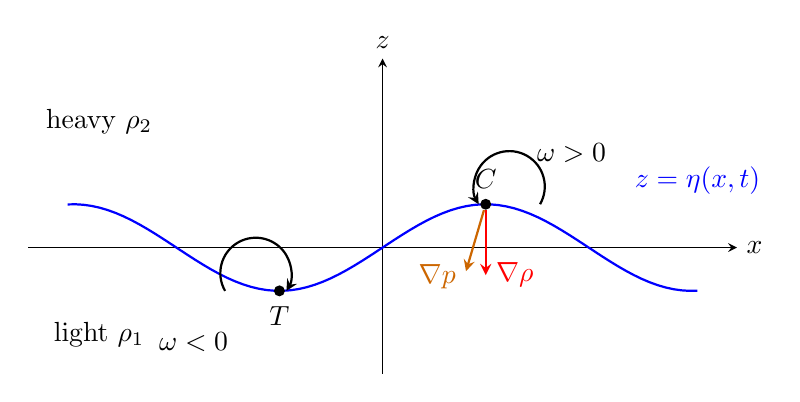
\begin{tikzpicture}[>=stealth, scale=1.0]
  % axes
  \draw[->] (-4.5,0) -- (4.5,0) node[right] {$x$};
  \draw[->] (0,-1.6) -- (0,2.4) node[above] {$z$};
  % perturbed interface
  \draw[thick, blue] plot[domain=-4:4, samples=80] (\x, {0.55*sin(deg(\x*1.2))});
  \node[blue, above] at (4.0, 0.55) {$z=\eta(x,t)$};
  % heavy/light labels
  \node at (-3.6, 1.6) {heavy $\rho_2$};
  \node at (-3.6,-1.1) {light $\rho_1$};
  % crest and trough markers
  \node[circle,fill,inner sep=1.4pt,label=above:{$C$}] (CR) at ({1.31},{0.55}) {};
  \node[circle,fill,inner sep=1.4pt,label=below:{$T$}] (TR) at ({-1.31},{-0.55}) {};
  % gradient arrows at crest C
  \draw[->, red, thick] (CR) -- ++(0,-0.9) node[right] {$\nabla\rho$};
  \draw[->, orange!80!black, thick] (CR) -- ++(-0.25,-0.85) node[left, yshift=-2pt] {$\nabla p$};
  % vorticity sign labels
  \node at (2.4, 1.2) {$\omega>0$};
  \node at (-2.4,-1.2) {$\omega<0$};
  % induced circulation arrows
  \draw[->, thick] (2.0, 0.55) arc[start angle=-30, end angle=210, radius=0.45];
  \draw[->, thick] (-2.0,-0.55) arc[start angle=210, end angle=-30, radius=0.45];
\end{tikzpicture}
\end{center}

\paragraph{Variation of $\sigma_n$ with $n$.} Energy argument: KE $\sim (\rho_1+\rho_2)v^2/(2k_n)$; PE released $\sim (\rho_2-\rho_1)g\eta^2/2$. Equate, with $v\sim\sigma\eta$:
\[ \sigma_n^2 \sim \frac{\rho_2-\rho_1}{\rho_1+\rho_2}\,g\,k_n. \]
Short waves (large $n$) localise motion at the interface where the baroclinic torque acts: faster growth. Finite depth $h$ caps the inertia at $\sim h$ once $k_n h\lesssim 1$, suppressing $\sigma_n$ by $\tanh(k_n h)$.

%==================================================================
\section*{Question 4 --- Stokes flow past a clean bubble}

\textbf{Problem.} (a) Derive $\nabla^2 p,\nabla^2\bm\omega\approx 0$ in Stokes flow; (b) verify incompressibility of axisymmetric streamfunction and write BCs at the bubble; (c) verify $\Psi=Cr\sin^2\theta$ and obtain drag $4\pi\eta a U$; (d) shrinking bubble at terminal velocity, find $a(z)$ and critical depth $d$ for $a_0=10^{-4}\,$m.

\subsection*{(a)}

Low-Re conditions: $\mathrm{Re}=UL/\nu\ll 1$; small $U$, small $L$, or large $\nu$. Examples: bacterial swimming, microfluidics, lava/honey flow.

Drop inertia in Navier--Stokes:
\[ 0 \approx -\nabla p + \eta\nabla^2\vb u + \rho\vb g. \]
Absorb gravity into modified pressure $p\to p+\rho g z$. Take divergence, use $\nabla\!\cdot\!\vb u=0$:
\[ \boxed{\;\nabla^2 p \approx 0.\;} \]
Take curl, use $\nabla\times\nabla p=0$ and $\nabla\times\nabla^2\vb u=\nabla^2\bm\omega$:
\[ \boxed{\;\nabla^2\bm\omega \approx 0.\;} \]

\subsection*{(b)}

Axisymmetric divergence:
\[ \nabla\!\cdot\!\vb v = \frac{1}{r^2}\pd{(r^2 v_r)}{r} + \frac{1}{r\sin\theta}\pd{(\sin\theta\,v_\theta)}{\theta}. \]
Substitute streamfunction definitions:
\[ \nabla\!\cdot\!\vb v = \frac{1}{r^2\sin\theta}\,\frac{\partial^2\Psi}{\partial r\,\partial\theta} - \frac{1}{r^2\sin\theta}\,\frac{\partial^2\Psi}{\partial\theta\,\partial r}. \]
Schwarz cancellation:
\[ \nabla\!\cdot\!\vb v = 0\ \checkmark. \]

\paragraph{BCs at the bubble.} No-penetration at $r=a$ (bubble-rest frame, far field $-U\hat{\vb z}$):
\[ v_r(a,\theta) = 0,\qquad v_r\to -U\cos\theta,\ v_\theta\to U\sin\theta\ \text{as}\ r\to\infty. \]
Inviscid interior $\Rightarrow$ tangential viscous stress vanishes:
\[ \sigma_{r\theta}\big|_{r=a} = 2\eta\,e_{r\theta}\big|_{r=a} = 0. \]
Use $v_r(a,\theta)=0\Rightarrow \partial v_r/\partial\theta|_{a}=0$:
\[ \boxed{\;\pd{}{r}\!\left(\frac{v_\theta}{r}\right)\bigg|_{r=a} = 0.\;} \]

\subsection*{(c)}

Full streamfunction (uniform far-field plus given correction):
\[ \Psi = -\tfrac12 U r^2\sin^2\theta + C r\sin^2\theta. \]
Compute $v_r$:
\[ v_r = \frac{1}{r^2\sin\theta}\pd{\Psi}{\theta} = -U\cos\theta + \frac{2C\cos\theta}{r}. \]
Compute $v_\theta$:
\[ v_\theta = -\frac{1}{r\sin\theta}\pd{\Psi}{r} = U\sin\theta - \frac{C\sin\theta}{r}. \]
Apply $v_r(a,\theta)=0$:
\[ C = \frac{Ua}{2}. \]
Form $v_\theta/r$ and differentiate:
\[ \pd{}{r}\!\left(\frac{v_\theta}{r}\right) = -\frac{U\sin\theta}{r^2} + \frac{2C\sin\theta}{r^3}. \]
Evaluate at $r=a$ with $C=Ua/2$:
\[ \pd{}{r}\!\left(\frac{v_\theta}{r}\right)\bigg|_{r=a} = -\frac{U\sin\theta}{a^2} + \frac{U\sin\theta}{a^2} = 0\ \checkmark. \]
Far-field matching at $r\to\infty$:
\[ v_r \to -U\cos\theta\ \checkmark. \]

\paragraph{Drag.} $z$-component of surface stress:
\[ T_z = (-p + 2\eta e_{rr})\cos\theta - 2\eta e_{r\theta}\sin\theta. \]
Tangential stress vanishes at $r=a$:
\[ 2\eta e_{r\theta}\big|_{r=a} = 0. \]
Compute $\partial v_r/\partial r$ at $r=a$ using $C=Ua/2$:
\[ \pd{v_r}{r}\bigg|_{r=a} = -\frac{2C\cos\theta}{a^2} = -\frac{U\cos\theta}{a}. \]
Hence radial viscous stress at the surface:
\[ 2\eta e_{rr}\big|_{r=a} = -\frac{2\eta U\cos\theta}{a}. \]
Pressure on the surface (given form, $r=a$):
\[ p\big|_{r=a} = p_0 + \frac{\eta U\cos\theta}{a}. \]
Combine:
\[ T_z\big|_{r=a} = -p_0\cos\theta - \frac{3\eta U\cos^2\theta}{a}. \]
Integrate over the sphere:
\[ F = 2\pi a^2\!\int_0^\pi\!\!\left[-p_0\cos\theta - \frac{3\eta U\cos^2\theta}{a}\right]\!\sin\theta\,\de\theta. \]
$\int_0^\pi\cos\theta\sin\theta\,\de\theta = 0$:
\[ F = -2\pi a^2\cdot\frac{3\eta U}{a}\cdot\int_0^\pi\!\cos^2\theta\sin\theta\,\de\theta. \]
Evaluate $\int_0^\pi\cos^2\theta\sin\theta\,\de\theta = 2/3$:
\[ F = -4\pi\eta a U. \]
Magnitude:
\[ \boxed{\;|F| = 4\pi\eta a U.\;} \]
($2/3$ of Stokes drag on rigid sphere; tangential stress missing at the free surface.)

\subsection*{(d)}

Terminal velocity: buoyancy = drag (with $\rho_a\ll\rho_w$):
\[ \tfrac{4}{3}\pi a^3 \rho_w g = 4\pi\eta_w a\,U. \]
Solve:
\[ U(a) = \frac{\rho_w g\,a^2}{3\eta_w}. \]
Mass: $M=\tfrac{4}{3}\pi a^3\rho_a$, so:
\[ \dv{M}{t} = 4\pi a^2\rho_a\dv{a}{t}. \]
Equate to dissolution rate $-4\pi a D_a\rho_a$:
\[ a\dv{a}{t} = -D_a. \]
Convert to $z$ via $\de z/\de t = U$:
\[ a\,U(a)\,\dv{a}{z} = -D_a. \]
Substitute $U(a)$:
\[ \frac{\rho_w g}{3\eta_w}\,a^3\,\dv{a}{z} = -D_a. \]
Separate and integrate from $a_0$ at $z=0$:
\[ \frac{\rho_w g}{3\eta_w}\!\int_{a_0}^{a}\!a'^3\,\de a' = -D_a\,z. \]
Evaluate:
\[ \frac{\rho_w g}{12\eta_w}\!\left(a^4 - a_0^4\right) = -D_a\,z. \]
Rearrange:
\[ \boxed{\;a^4(z) = a_0^4 - \frac{12\eta_w D_a}{\rho_w g}\,z.\;} \]

\paragraph{Critical depth.} Set $a(d)=0$:
\[ d = \frac{\rho_w g\,a_0^4}{12\,\eta_w D_a}. \]
Numerical evaluation: $a_0=\SI{e-4}{m}$, $\rho_w=\SI{e3}{kg.m^{-3}}$, $g=\SI{9.81}{m.s^{-2}}$, $\eta_w=\SI{e-3}{Pa.s}$, $D_a=\SI{e-10}{m^2.s^{-1}}$.

Numerator:
\[ \rho_w g\,a_0^4 = (10^3)(9.81)(10^{-4})^4 = 9.81\times 10^{-13}\ \text{kg\,m}^{-1}\text{s}^{-2}\cdot\text{m}^4. \]
Denominator:
\[ 12\,\eta_w D_a = 12\,(10^{-3})(10^{-10}) = 1.2\times 10^{-12}. \]
Divide:
\[ d = \frac{9.81\times 10^{-13}}{1.2\times 10^{-12}}\,\text{m}. \]
\[ \boxed{\;d \approx \SI{0.82}{m}.\;} \]

\end{document}
